\documentclass[10pt, a5paper]{article}
\usepackage{ucs}
\usepackage[utf8]{inputenc}
\usepackage[T2A]{fontenc}
\usepackage[english, russian]{babel}
\usepackage{hyperref}
\usepackage{geometry}
\usepackage{graphicx}
\frenchspacing

\begin{document}
\renewcommand{\figurename}{Рыс.} % Не перакідаць у прэамбулу --- не працуе, чаму -- халера ведае.
\renewcommand{\abstractname}{Анатацыя}
\renewcommand{\refname}{Літаратура}

\title{Выкарыстання вольнага праграмнага забеспячэння ва ўстановах адукацыі Украіны: спроба аналізу}

\author{Грыгорый Злобiн\\
\small Львоўскі нацыянальны універсітэт ім. Івана Франка,\\
\small \texttt{zlobin@electronics.wups.lviv.ua}
}
\date{}

\maketitle

\begin{abstract}
The analysis of free / open source software usage in higher educational institutions of Ukraine is presented, based of the ``FOSS Lviv-2011''  International Scientific Conference reports. 
\end{abstract}

Нягледзячы на станоўчы досвед выкарыстання вольнага праграмнага забеспячэння (СПЗ) у адукацыі як у краінах блізкага, так і далёкага замежжа ў Украіну да гэтага часу не прынята канцэпцыя выкарыстання СПЗ у адукацыі. Разам з тым намаганнямі энтузіястаў у навучальных установах Украіны свабоднае праграмнае забеспячэнне ўсё ж выкарыстоўваецца! Праз адхіленую пазіцыю міністэрства адукацыі і навукі Украіны няма падрабязнай інфармацыі аб вопыце выкарыстання СПО у адукацыі. Дзякуючы таму, што ў Львоўскім нацыянальным універсітэце імя Івана Франка 01--06 люты 2011 адбылася даволі прадстаўнічая міжнародная навукова-практычная канферэнцыя <<FOSS Lviv-2011>>, з'явілася магчымасць правядзення аналізу выкарыстання СПЗ у вышэйшых навучальных установах Украіны. З 81 дакладаў 49 было прысвечана выкарыстанню СПО ў навучальных установах. Даклады \cite{fosslviv}, якія былі пададзеныя на гэтую канферэнцыю можна згрупаваць па наступных кірунках (назва дакладу падаецца на мове арыгіналу):

\section{Дыстанцыйнае навучанне}

Гэтай тэматыцы прысвечана найбольшая колькасць дакладаў --- 10:
\begin{itemize}
\item <<Розроблення електронного деканату для системи управління дистанційним навчання MOODLE>> --- Артеменко В.Б., Львоўская камерцыйная акадэмія
\item <<Вибір платформи дистанційного навчання>> --- Коцаренко М.В., Бойко О.В.,  Львоўскі нацыянальны медыцынскі універсітэт ім. Данііла Галіцкага
\item <<Використання контрольно-діагностичної програми iTest у ході моніторингу якості процесу навчання старшокласників>> --- Макаренко І.Є., Мерзлікін П.В., Крыварожскі дзяржаўны педагагічны універсітэт
\item  <<Використання системи Moodle для організації контролю знань майбутніми вчителями-гуманітаріями>> --- Маркова Є.С., Бердянскі дзяржаўны педагагічны універсітэт
\item  <<Тестування в  Moodle як елемент менеджменту якості освіти: перший досвід>> --- Сергієнко В.П., Сліпухіна І.А., НПУ ім. М.П. Драгоманова
\item  <<Особливості програмного забезпечення в електронному навчанні>> --- Жарких Ю.С., Лисоченко С.В., Сусь Б.Б., Третяк О.В., Кіеўскі нацыянальны універсітэт ім. Тараса Шевченка
\item  <<Інформаційно-аналітична система управління навчальним процесом ВНЗ на базі  Moodle>> --- Триус Ю.В., Чаркаскі дзяржаўны тэхналагічны універсітэт
\item  <<Використання CMS JOMLA!  та LCMS MOODLE у ВНЗ>> --- Франчук В.М., НПУ ім. М.П. Драгоманова
\item <<Локалізація системи MOODLE " --- Франчук В.М., НПУ ім. М.П. Драгоманова
\item  <<Застосування вільного програмного забезпечення для дистанційного навчання у вищих навчальних закладах>> --- Захарченко В.М., Шапо В.М., Адэская нацыянальная марская акадэмія
\end{itemize}

\section{Выкарыстанне сістэм камп'ютэрнай матэматыкі}
Наступныя 6 дакладаў могуць быць аднесены да матэматычнай тэматыцы:
\begin{itemize}
\item <<Використання вільно-поширюваного ПЗ математичного призначення в університеті>> --- Бугаєць Н.О., НПУ ім. М.П. Драгоманова
\item <<Вільнопоширювані системи комп'ютерної математики в освіті і науці>> --- Лазурчак І.І., Кобильник Т.П., Драгобыцкі дзяржаўны універсітэт ім.  І. Франка
\item <<Використання комп'ютерних математичних систем у професійній підготовці майбутнього вчителя математики>> --- Лов'янова І.В., Крыварожскі дзяржаўны педагагічны універсітэт
\item <<Моделювання задач електротехніки у XCOS>> --- Філь І.М., Данецкі нацыянальны тэхнічны універсітэт
\item <<Розробка і використання web-інтерфейсів для роботи з системами комп'ютерної математики>> --- Чичкарьов Є.А., Приазовскі дзяржаўны тэхнічны універсітэт
\item <<Про комп'ютерний супровід викладання геометрії>> --- Яхненко І.В., Лутфулін М.В., Палтаўскі нацыянальны педагагічны універсітэт ім. В.Г. Короленка
\end{itemize}

\section{Агульныя пытанні выкарыстання СПЗ у адукацыі}
7 дакладаў гэтай групы, якую можна прызнаць другой па колькасці, ўключалі:
\begin{itemize}
\item <<Використання вільного програмного забезпечення в навчанні і наукових дослідженнях у Львівському національному університеті імені Івана Франка>> --- Апуневич С.Є., Злобін Г.Г., Рикалюк Р.Є., Шувар Р.Я., Львоўскі нацыяналь-ны універсітэт ім. І. Франка
\item <<Використання вільного програмного забезпечення в системі дистанційної освіти>> --- Воронкін О.С., Луганскі дзяржаўны інстытут культуры і мастацтваў
\item <<Вільнопоширюване програмне забезпечення курсу “Нові інформаційні технології” для студентів спеціальності “Біологія”>> --- Єфименко В.В., НПУ ім. М.П. Драгоманова
\item <<Використання вільного програмного забез-печення у професійній підготовці майбутніх інженерів>> --- Покришень Д.А., Дрозд О.П., Сподаренко І.Й., Чарнігаўскі дзяржаўны тэхналагічны універсітэт
\item  <<Про досвід використання ОС Linux у навчальному процесі Львівського національного медичного університету імені Данила Галицького>> --- Риковський П.А., Львоўскі нацыянальны медыцынскі універсітэт ім. Данііла Галіцкага
\item  <<LINUX  та VIRTUAL-BOX у навчанні абстрактних понять теорії операційних систем>> --- Спірін О.М., Сверчевська О.С., Жытомірскі дзяржаўны універсітэт ім. І. Франка
\item  <<З досвіду використання вільного програмного забезпечення при вивченні інформатики>> --- Харченко В.М., Нежынскі дзяржаўны універсітэт ім. М. Гогаля
\end{itemize}

\section{Выкарыстаньне адкрытых сродкаў праграмавання}
Дадзеная група апынулася найменшай па колькасці і ўключае 4 даклада:
\begin{itemize}
\item <<Використання відкритих програмних засобів в процесі навчання статистичним дисциплінам>> --- Коркуна Т.Й., Самбарскі тэхнікум эканомікі і інфарматыкі
\item <<Розрахунок фотоіонізаційних моделей небулярного газу в ОС LINUX UBUNTU 10.10 та WINDOWS 7>> --- Мелех Б.Я., Тишко Н.Л., Коритко Р.І., Львоўскі нацыянальны  універсітэт ім. І. Франка
\item <<Реалізація розподілених обчислень на основі грід-платформи з відкритим кодом BOINC>> --- Шийка Ю.Я., Шувар Р.Я., Львоўскі нацыянальны  універсітэт ім. І. Франка
\item <<Реалізація високопродуктивної обчислювальної системи на базі ОС  LINUX>> --- Шувар Р.Я., Бойко Я.В., Львоўскі нацыянальны  універсітэт ім. І. Франка
\end{itemize}

\section{Распрацоўка праграмнага забеспячэння}
Будучы тэматычна-роднаснай папярэдняй, дадзеная група больш шматлікая і складаецца з 7 дакладаў, зраўнаваўся з катэгорыяй <<Агульныя пытанні выкарыстання СПЗ у адукацыі>>:
\begin{itemize}
\item <<Комплекс програм для лазерних спостережень штучних супутників Землі>> --- Мартинюк-Лотоцький К.П., Білінський А.І., Львоўскі нацыянальны  універсітэт ім. І. Франка
\item <<Розробка системи спектральної діагностики димової плазми>> --- Сподарець Д.В., Драган Г.С., Адэскі нацыянальны універсітэт імя І.І. Мечнікава
\item <<Використання вільного програмного забез-печення для створення програми керування інформаційним автоматом>> --- Злобін Г., Скляр В., Чмихало О., Шевчик В., Львоўскі нацыянальны  універсітэт ім. І. Франка
\item <<Використання бібліотеки класів GEANT4 в ОС Linux при розробці програмного забезпечення для моделювання процесів взаємодії випромінювання з речовиною>> --- Малихіна Т.В., Харкаўскі нацыяналь-ны універсітэт ім. В.Н. Каразина
\item  <<Програма для обробкирезультатів ЛЛС-спостережень як ВПЗ>> --- Апуневич С.Є., Апуневич С.В., Білінський А.І., Благодир Я.Т., Львоўскі нацыянальны  універсітэт ім. І. Франка
\item  <<Програмне забезпечення керування телескопом  ЛЛС-станції Львів-1831>> --- Білінський А.І., Мартинюк-Лотоцький К.П., Львоўскі нацыянальны  універсітэт ім. І. Франка
\item <<Використання Open Wrt як основи вбудованого програмного забезпечення маршрутизаторів>> --- Нек Т., Львоўскі нацыянальны  універсітэт ім. І. Франка
\end{itemize}

\section{Асобныя даклады}
І нарэшце, 5 дакладаў не могуць быць аднесены ні да адной з пералічаных вышэй катэгорый:
\begin{itemize}
\item  <<Інформаційна технологія управління навчальним навантаженням у вищих навчальних закладах>> --- Гриценко В.Г., Чаркаскі нацыянальны універсітэт  ім. Б. Хмяльніцкага
\item  <<Про досвід використання офісного  пакету OpenOffice.org.ukr в курсі інформатики для економічних і юридичних спеціальностей ВЗО>> --- Злобін Г.Г., Львоўскі нацыянальны універсітэт ім. І. Франка 
\item  <<Досвід використання  редактора Gimp при вивченні курсу “Комп'ютерна графіка і дизайн”>> --- Матвієнко Ю.С., Палтаўскі нацыянальны педагагічны універсітэт ім.  В.Г. Короленка
\item <<Використання програми GANTTPROJECT для побудови календарних графіків при розробці ПВР>> --- Грицук Ю.В., Меліхов О.І., Данбаская акадэмія будаўніцтва і архітэктуры
\item <<Вільне ПЗ для підготовки наукових текстів і презентацій>> --- Лутфуллін М.В., Моторний М.І., Палтаўскі нацыянальны педагагічны універсітэт ім.  В.Г. Короленка
\end{itemize}

	Такім чынам можна канстатаваць як шырокі спектр выкарыстання СПЗ ва ўкраінскіх навучальных установах ад дыстанцыйнага навучання да распрацоўцы адкрытага праграмнага забеспячэння, так і шырокую геаграфію выкарыстання СПЗ ад Луганска на ўсходзе ў Львоў на захадзе і ад Чарнігава на поўначы да Адэсы на поўдні (глядзі рыс.).

\begin{figure}[ht]
\centering{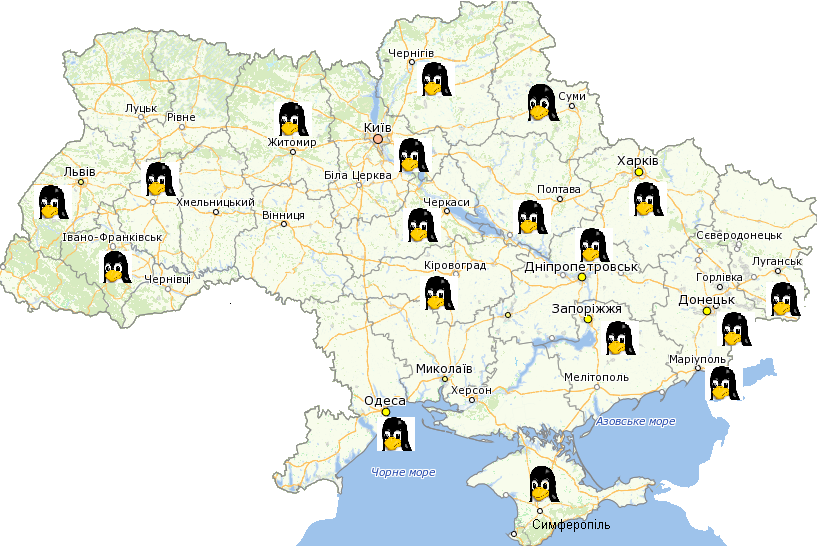
\includegraphics[width=8cm]{05_ukraine_linux.png}}
\label{pic:fl1}
%\caption{~}
\end{figure}

\begin{thebibliography}{9}
\bibitem{fosslviv}Тези міжнародної науково-практичної конференції FOSS LVIV-2011. Збірник наукових праць /за ред. Злобіна Г.Г., Апуневича С.Є., Машкова В.В., Апуневич С.В. Вид-во ЛНУ імені Івана Франка. 2011. --- 196 с.
\end{thebibliography}

\end{document}




